\documentclass[aspectratio=169,12pt]{beamer}

% --- Tema y colores -------------------------------------------------------------------
\usetheme{Madrid}
\usecolortheme{default}

\definecolor{azulUNSAAC}{RGB}{0,51,102}
\definecolor{dorado}{RGB}{204,153,0}
\definecolor{verdeDark}{RGB}{0,102,68}
\definecolor{rojoAlerta}{RGB}{180,30,30}
\definecolor{grisCla}{RGB}{245,245,250}
\definecolor{grisOsc}{RGB}{60,60,80}

\setbeamercolor{palette primary}{bg=azulUNSAAC, fg=white}
\setbeamercolor{palette secondary}{bg=azulUNSAAC!80, fg=white}
\setbeamercolor{palette tertiary}{bg=azulUNSAAC!60, fg=white}
\setbeamercolor{palette quaternary}{bg=azulUNSAAC, fg=white}
\setbeamercolor{structure}{fg=azulUNSAAC}
\setbeamercolor{block title}{bg=azulUNSAAC, fg=white}
\setbeamercolor{block body}{bg=grisCla}
\setbeamercolor{block title alerted}{bg=rojoAlerta, fg=white}
\setbeamercolor{block body alerted}{bg=red!5}
\setbeamercolor{block title example}{bg=verdeDark, fg=white}
\setbeamercolor{block body example}{bg=green!5}
\setbeamercolor{frametitle}{bg=azulUNSAAC, fg=white}
\setbeamercolor{title}{fg=white}
\setbeamercolor{subtitle}{fg=dorado}

% --- Paquetes -------------------------------------------------------------------------
\usepackage[utf8]{inputenc}
\usepackage[T1]{fontenc}
\usepackage{lmodern}
\usepackage[spanish]{babel}
\usepackage{booktabs}
\usepackage{multirow}
\usepackage{array}
\usepackage{colortbl}
\usepackage{tikz}
\usetikzlibrary{shapes,arrows.meta,positioning,calc}
\usepackage{pgfplots}
\pgfplotsset{compat=1.18}
\usepackage{amsmath,amssymb}
\usepackage{pifont}
\usepackage{graphicx}
\usepackage{xcolor}
\usepackage{caption}

% --- Configuracion de listas -------------------------------------------------------
\setbeamertemplate{itemize items}[circle]
\setbeamertemplate{enumerate items}[default]
\setbeamertemplate{navigation symbols}{}

% --- Comandos utilitarios ---------------------------------------------------------
\newcommand{\highlight}[1]{\textcolor{dorado}{\textbf{#1}}}
\newcommand{\alerttext}[1]{\textcolor{rojoAlerta}{\textbf{#1}}}
\newcommand{\oktext}[1]{\textcolor{verdeDark}{\textbf{#1}}}
\newcommand{\complejidad}[1]{\ensuremath{\mathcal{O}\!\left(#1\right)}}
\newcolumntype{C}[1]{>{\centering\arraybackslash}p{#1}}

% --- Metadatos -------------------------------------------------------------------
\title[SSSP: Dijkstra, Bellman-Ford, DMMSY]{\textbf{Caminos Más Cortos con Fuente Única}\\
\large Comparación Experimental: Dijkstra, Bellman-Ford,\\Thorup y el Algoritmo Determinista \complejidad{m \log^{2/3} n}}
\subtitle{Algoritmos Avanzados --- Ingeniería Informática y de Sistemas}
\author[Bustinza · Mayhuire · Estacio · Salcedo]{
  José M.\ Bustinza Quispe \and Brenda L.\ Mayhuire Chacón \\[2pt]
  Amilcar Estacio Medrano \and Mirco S.\ Salcedo Ataulluco
}
\institute[UNSAAC]{Universidad Nacional de San Antonio Abad del Cusco\\
\textit{Facultad de Ingeniería Informática y de Sistemas}}
\date{Junio 2026}

% --- Logo -----------------------------------------------------------------------
% \logo{\includegraphics[height=0.7cm]{unsaac_logo.png}}

% ══════════════════════════════════════════════════════════════════════════════
\begin{document}
% ══════════════════════════════════════════════════════════════════════════════

% --- Portada ------------------------------------------------------------------
{
\setbeamertemplate{headline}{}
\begin{frame}[plain]
  \begin{tikzpicture}[remember picture, overlay]
    \fill[azulUNSAAC] (current page.north west) rectangle
      ([yshift=-2.5cm]current page.north east);
    \fill[dorado] ([yshift=-2.5cm]current page.north west) rectangle
      ([yshift=-2.75cm]current page.north east);
    \node[white, font=\Large\bfseries, anchor=west]
      at ([xshift=1cm, yshift=-1.25cm]current page.north west)
      {UNSAAC \textbullet{} Algoritmos Avanzados};
  \end{tikzpicture}
  \vspace{1.5cm}
  \titlepage
\end{frame}
}

% --- Tabla de contenidos --------------------------------------------------
\begin{frame}{Contenido de la Presentación}
\small
\begin{columns}[t]

\column{0.48\textwidth}
\tableofcontents[
  hideallsubsections,
  sections={1-5}
]

\column{0.48\textwidth}
\tableofcontents[
  hideallsubsections,
  sections={6-10}
]

\end{columns}
\end{frame}

% ===============================================================================
\section{Introducción y Motivación}
% ===============================================================================

\begin{frame}{El Problema SSSP}
  \begin{columns}[T]
    \begin{column}{0.5\textwidth}
      \begin{block}{Definición formal}
        Dado $G=(V,E)$ dirigido con pesos enteros no negativos y origen $s\in V$,
        encontrar la distancia mínima $d(v)$ desde $s$ hacia todo $v\in V$.
      \end{block}
      \vspace{0.25cm}
      \textbf{Aplicaciones directas:}
      \begin{itemize}
        \item Navegación GPS y sistemas de ruteo
        \item Diseño de redes de comunicación
        \item Análisis de redes sociales (centralidad)
        \item Planificación logística
      \end{itemize}
    \end{column}
    \begin{column}{0.35\textwidth}
      \begin{tikzpicture}[scale=1.0,xshift=1.5cm,
        nd/.style={circle,draw=azulUNSAAC,fill=azulUNSAAC!15,
                   font=\small\bfseries,minimum size=7mm},
        src/.style={circle,draw=dorado,fill=dorado!30,
                    font=\small\bfseries,minimum size=7mm,
                    line width=1.5pt}]
        \node[src] (s) at (0,0)   {s};
        \node[nd]  (a) at (2, 1)  {a};
        \node[nd]  (b) at (2,-1)  {b};
        \node[nd]  (c) at (4, 0)  {c};
        \node[nd]  (d) at (4,-2)  {d};
        \draw[->,thick,azulUNSAAC] (s)--(a) node[midway,above,font=\tiny]{3};
        \draw[->,thick,azulUNSAAC] (s)--(b) node[midway,below,font=\tiny]{1};
        \draw[->,thick,azulUNSAAC] (a)--(c) node[midway,above,font=\tiny]{2};
        \draw[->,thick,azulUNSAAC] (b)--(c) node[midway,above,font=\tiny]{4};
        \draw[->,thick,azulUNSAAC] (b)--(d) node[midway,below,font=\tiny]{5};
        \draw[->,thick,verdeDark,dashed,line width=1.5pt]
          (s)--(b) node[midway,above,font=\tiny,verdeDark]{};
        \draw[->,thick,verdeDark,dashed,line width=1.5pt]
          (s)--(a);
        \draw[->,thick,verdeDark,dashed,line width=1.5pt]
          (a)--(c);
      \end{tikzpicture}
      \vspace{0.2cm}
      \begin{center}\small\textcolor{verdeDark}{\textit{Caminos mínimos desde s}}\end{center}
    \end{column}
  \end{columns}
\end{frame}

\begin{frame}{Evolución Histórica del Problema}
\centering

\begin{tikzpicture}[
    font=\small,
    milestone/.style={
        rectangle,
        rounded corners=3pt,
        draw=azulUNSAAC,
        fill=azulUNSAAC!12,
        align=center,
        text width=3.2cm,
        minimum height=1.6cm
    },
    highlight/.style={
        rectangle,
        rounded corners=3pt,
        draw=dorado,
        fill=dorado!18,
        align=center,
        text width=3.2cm,
        minimum height=1.6cm
    },
    arrow/.style={
        -{Stealth[length=3mm]},
        thick,
        azulUNSAAC
    }
]

% FILA SUPERIOR
\node[milestone] (dijkstra) at (0,0)
{
\textbf{1959}\\
Dijkstra\\
$\mathcal{O}(m+n\log n)$
};

\node[milestone] (bellman) at (4.3,0)
{
\textbf{1956--1958}\\
Bellman--Ford\\
$\mathcal{O}(mn)$
};

\node[milestone] (fib) at (8.6,0)
{
\textbf{1987}\\
Fibonacci Heap\\
$\mathcal{O}(m+n\log n)$
};

% FILA INFERIOR
\node[milestone] (thorup) at (0,-3)
{
\textbf{1999}\\
Thorup\\
$\mathcal{O}(m+n)$\\
(no dirigido)
};

\node[highlight] (dmmsy) at (4.3,-3)
{
\textbf{2025}\\
DMMSY\\
$\mathcal{O}(m\log^{2/3}n)$
};

\node[milestone] (pettie) at (8.6,-3)
{
\textbf{2002}\\
Pettie--Ramachandran\\
Pesos reales
};

% FLECHAS
\draw[arrow] (dijkstra) -- (bellman);
\draw[arrow] (bellman) -- (fib);

\draw[arrow] (dijkstra) -- (thorup);
\draw[arrow] (fib) -- (pettie);

\draw[arrow] (thorup) -- (dmmsy);
\draw[arrow] (pettie) -- (dmmsy);

% MENSAJE CENTRAL
\node[
    dorado,
    font=\scriptsize\bfseries,
    align=center
] at (4.3,-4.35)
{
$\star$ Primer avance determinista\\
en más de 20 años
};

\end{tikzpicture}

\end{frame}

% ──────────────────────────────────────────────────────────────────────────────
\begin{frame}{Los Cuatro Algoritmos Evaluados}
  \begin{columns}[T]
    \begin{column}{0.48\textwidth}
      \begin{block}{$\checkmark$~Implementaciones \textit{completas}}
        \begin{tabular}{@{}ll@{}}
          \textbf{Dijkstra} & \complejidad{(m+n)\log n}\\[2pt]
          \textbf{Bellman-Ford} & \complejidad{m\cdot n}\\
        \end{tabular}
      \end{block}
      \vspace{0.2cm}
      \begin{exampleblock}{$\star$~Implementaciones \textit{educativas}}
        \begin{tabular}{@{}ll@{}}
          \textbf{Thorup} & \complejidad{m+\sqrt{w_{\max}\cdot n}}\\[2pt]
          \textbf{DMMSY} & 1 nivel, \complejidad{m+D/w_0}\\
        \end{tabular}
      \end{exampleblock}
    \end{column}
    \begin{column}{0.48\textwidth}
      \small
      \begin{alertblock}{!!~Nota importante}
        Thorup y DMMSY capturan la \textbf{idea central} de cada algoritmo pero
        \emph{no} constituyen implementaciones completas de los papers originales:
        solo para fines pedagógicos.
      \end{alertblock}
      \vspace{0.2cm}
      \textbf{Pregunta de investigación:}\\
      ¿Cómo afecta la \textbf{densidad} $m/n$ al rendimiento relativo de los cuatro algoritmos?
    \end{column}
  \end{columns}
\end{frame}

% ===============================================================================
\section{Entorno y Metodología Experimental}
% ===============================================================================

\begin{frame}{Entorno Experimental}
  \begin{columns}[T]
    \begin{column}{0.48\textwidth}
      \textbf{$\blacksquare$~Hardware}
      \begin{itemize}\small
        \item Intel Core i5-1035G1 @ 1.00\,GHz (4C/8T)
        \item 16\,GB RAM
        \item SSD Kingston SNV2S500G 500\,GB
        \item Ejecución \textbf{monohilo}, sin paralelismo
        \item Medición: \texttt{std::chrono::high\_resolution\_clock}
        \item Resolución: $\approx 1\,\mu s$
      \end{itemize}
    \end{column}
    \begin{column}{0.48\textwidth}
      \textbf{$\blacksquare$~Software}
      \begin{itemize}\small
        \item g++ MinGW-w64 14.2.0, C++17, \texttt{-O2}
        \item Python 3.13 + pandas 2.3.2
        \item matplotlib 3.10.6, seaborn 0.13.2
        \item Git 2.43.0
      \end{itemize}
      \vspace{0.2cm}
      \textbf{$\blacksquare$~Grafos generados:}\\
      \small
      \texttt{generateRandomGraph(n, m, maxW, seed)}\\
      $w_{\max}=1\,000$, semilla fija $\Rightarrow$ \textbf{totalmente reproducibles}
    \end{column}
  \end{columns}
\end{frame}

% ──────────────────────────────────────────────────────────────────────────────
\begin{frame}{Diseño Experimental: Cuatro Experimentos}
  \begin{center}
  {\scriptsize
  \begin{tabular}{C{1.8cm}C{3.2cm}C{3.2cm}C{2.2cm}}
    \toprule
    \rowcolor{azulUNSAAC!20}
    \textbf{Exp.} & \textbf{Variable} & \textbf{Rango} & \textbf{Fijo}\\
    \midrule
    1 & Escalabilidad en $n$ & $n\in\{100,\ldots,10{,}000\}$ & $m=2n$\\
    \addlinespace[3pt]
    2 & Escalabilidad en $m$ & $m\in\{1{,}000,\ldots,200{,}000\}$ & $n=1{,}000$\\
    \addlinespace[3pt]
    3 & Densidades & $m\in\{500,2{,}500,12{,}500,50{,}000\}$ & $n=500$\\
    \addlinespace[3pt]
    \rowcolor{dorado!15}
    4 & \textbf{Aporte propio} & $n\times$ densidad (factorial) & 3 semillas\\
    \bottomrule
  \end{tabular}
  }
  \end{center}
  \vspace{0.15cm}
  \begin{columns}[T]
    \begin{column}{0.48\textwidth}
      {\footnotesize\textbf{Métricas recolectadas:}}
      \begin{enumerate}\scriptsize
        \item Tiempo de ejecución ($\mu s$)
        \item Operaciones de relajación (hardware-independiente)
      \end{enumerate}
    \end{column}
    \begin{column}{0.48\textwidth}
      {\footnotesize\textbf{Exp. 4 — niveles de densidad:}}
      \begin{itemize}\scriptsize
        \item \textit{muy\_disperso}: $m=n$
        \item \textit{disperso}: $m=2n$
        \item \textit{semi\_denso}: $m=5n$
        \item \textit{denso}: $m=10n$
        \item \textit{muy\_denso}: $m\approx n^2/4$
      \end{itemize}
    \end{column}
  \end{columns}
\end{frame}

% ──────────────────────────────────────────────────────────────────────────────
\begin{frame}{Hipótesis de Investigación}
  \begin{enumerate}
    \item[\textbf{H1}] \textbf{Dijkstra} es el más eficiente para grafos dispersos.
    \item[\textbf{H2}] \textbf{Bellman-Ford} es viable solo para $n\leq 500$.
    \item[\textbf{H3}] \textbf{Thorup} presenta el mayor tiempo por overhead de cubetas.
    \item[\textbf{H4}] \textbf{DMMSY} supera a Dijkstra en grafos de muy alta densidad.
  \end{enumerate}
\end{frame}

% ===============================================================================
\section{Resultados: Experimentos 1--3}
% ===============================================================================

\begin{frame}{Experimento 1 — Escalabilidad en $n$ (m = 2n)}
  \begin{columns}[T]
    \begin{column}{0.50\textwidth}
      \begin{center}
      \scriptsize
      \begin{tabular}{r r r r r r}
        \toprule
        \rowcolor{azulUNSAAC!20}
        $n$ & $m$ & \textbf{Dijk.} & \textbf{BF} & \textbf{DMMSY} & \textbf{Thorup}\\
         & & ($\mu s$) & ($\mu s$) & ($\mu s$) & ($\mu s$)\\
        \midrule
        100    & 200     & 10    & 11    & 106    & 960   \\
        500    & 1\,000  & 50    & 52    & 438    & 3\,127 \\
        1\,000 & 2\,000  & 129   & 102   & 1\,108 & 5\,779 \\
        2\,000 & 4\,000  & 244   & 251   & 1\,232 & 10\,877 \\
        5\,000 & 10\,000 & 581   & \textit{SKIP} & 3\,198 & 25\,742 \\
        \rowcolor{verdeDark!10}
        10\,000 & 20\,000 & \oktext{1\,380} & \textit{SKIP} & 7\,492 & 52\,209 \\
        \bottomrule
      \end{tabular}
      \end{center}
      \vspace{0.2cm}
      \scriptsize
      \begin{itemize}
        \item Dijkstra crece $138\times$ (factor $100\times$ en $n$)
        \item \highlight{Thorup}: overhead $\approx35$--$40\times$ sobre Dijkstra
        \item BF omitido para $n>2{,}000$ (coste cuadrático)
      \end{itemize}
    \end{column}
    \begin{column}{0.48\textwidth}
      \centering
      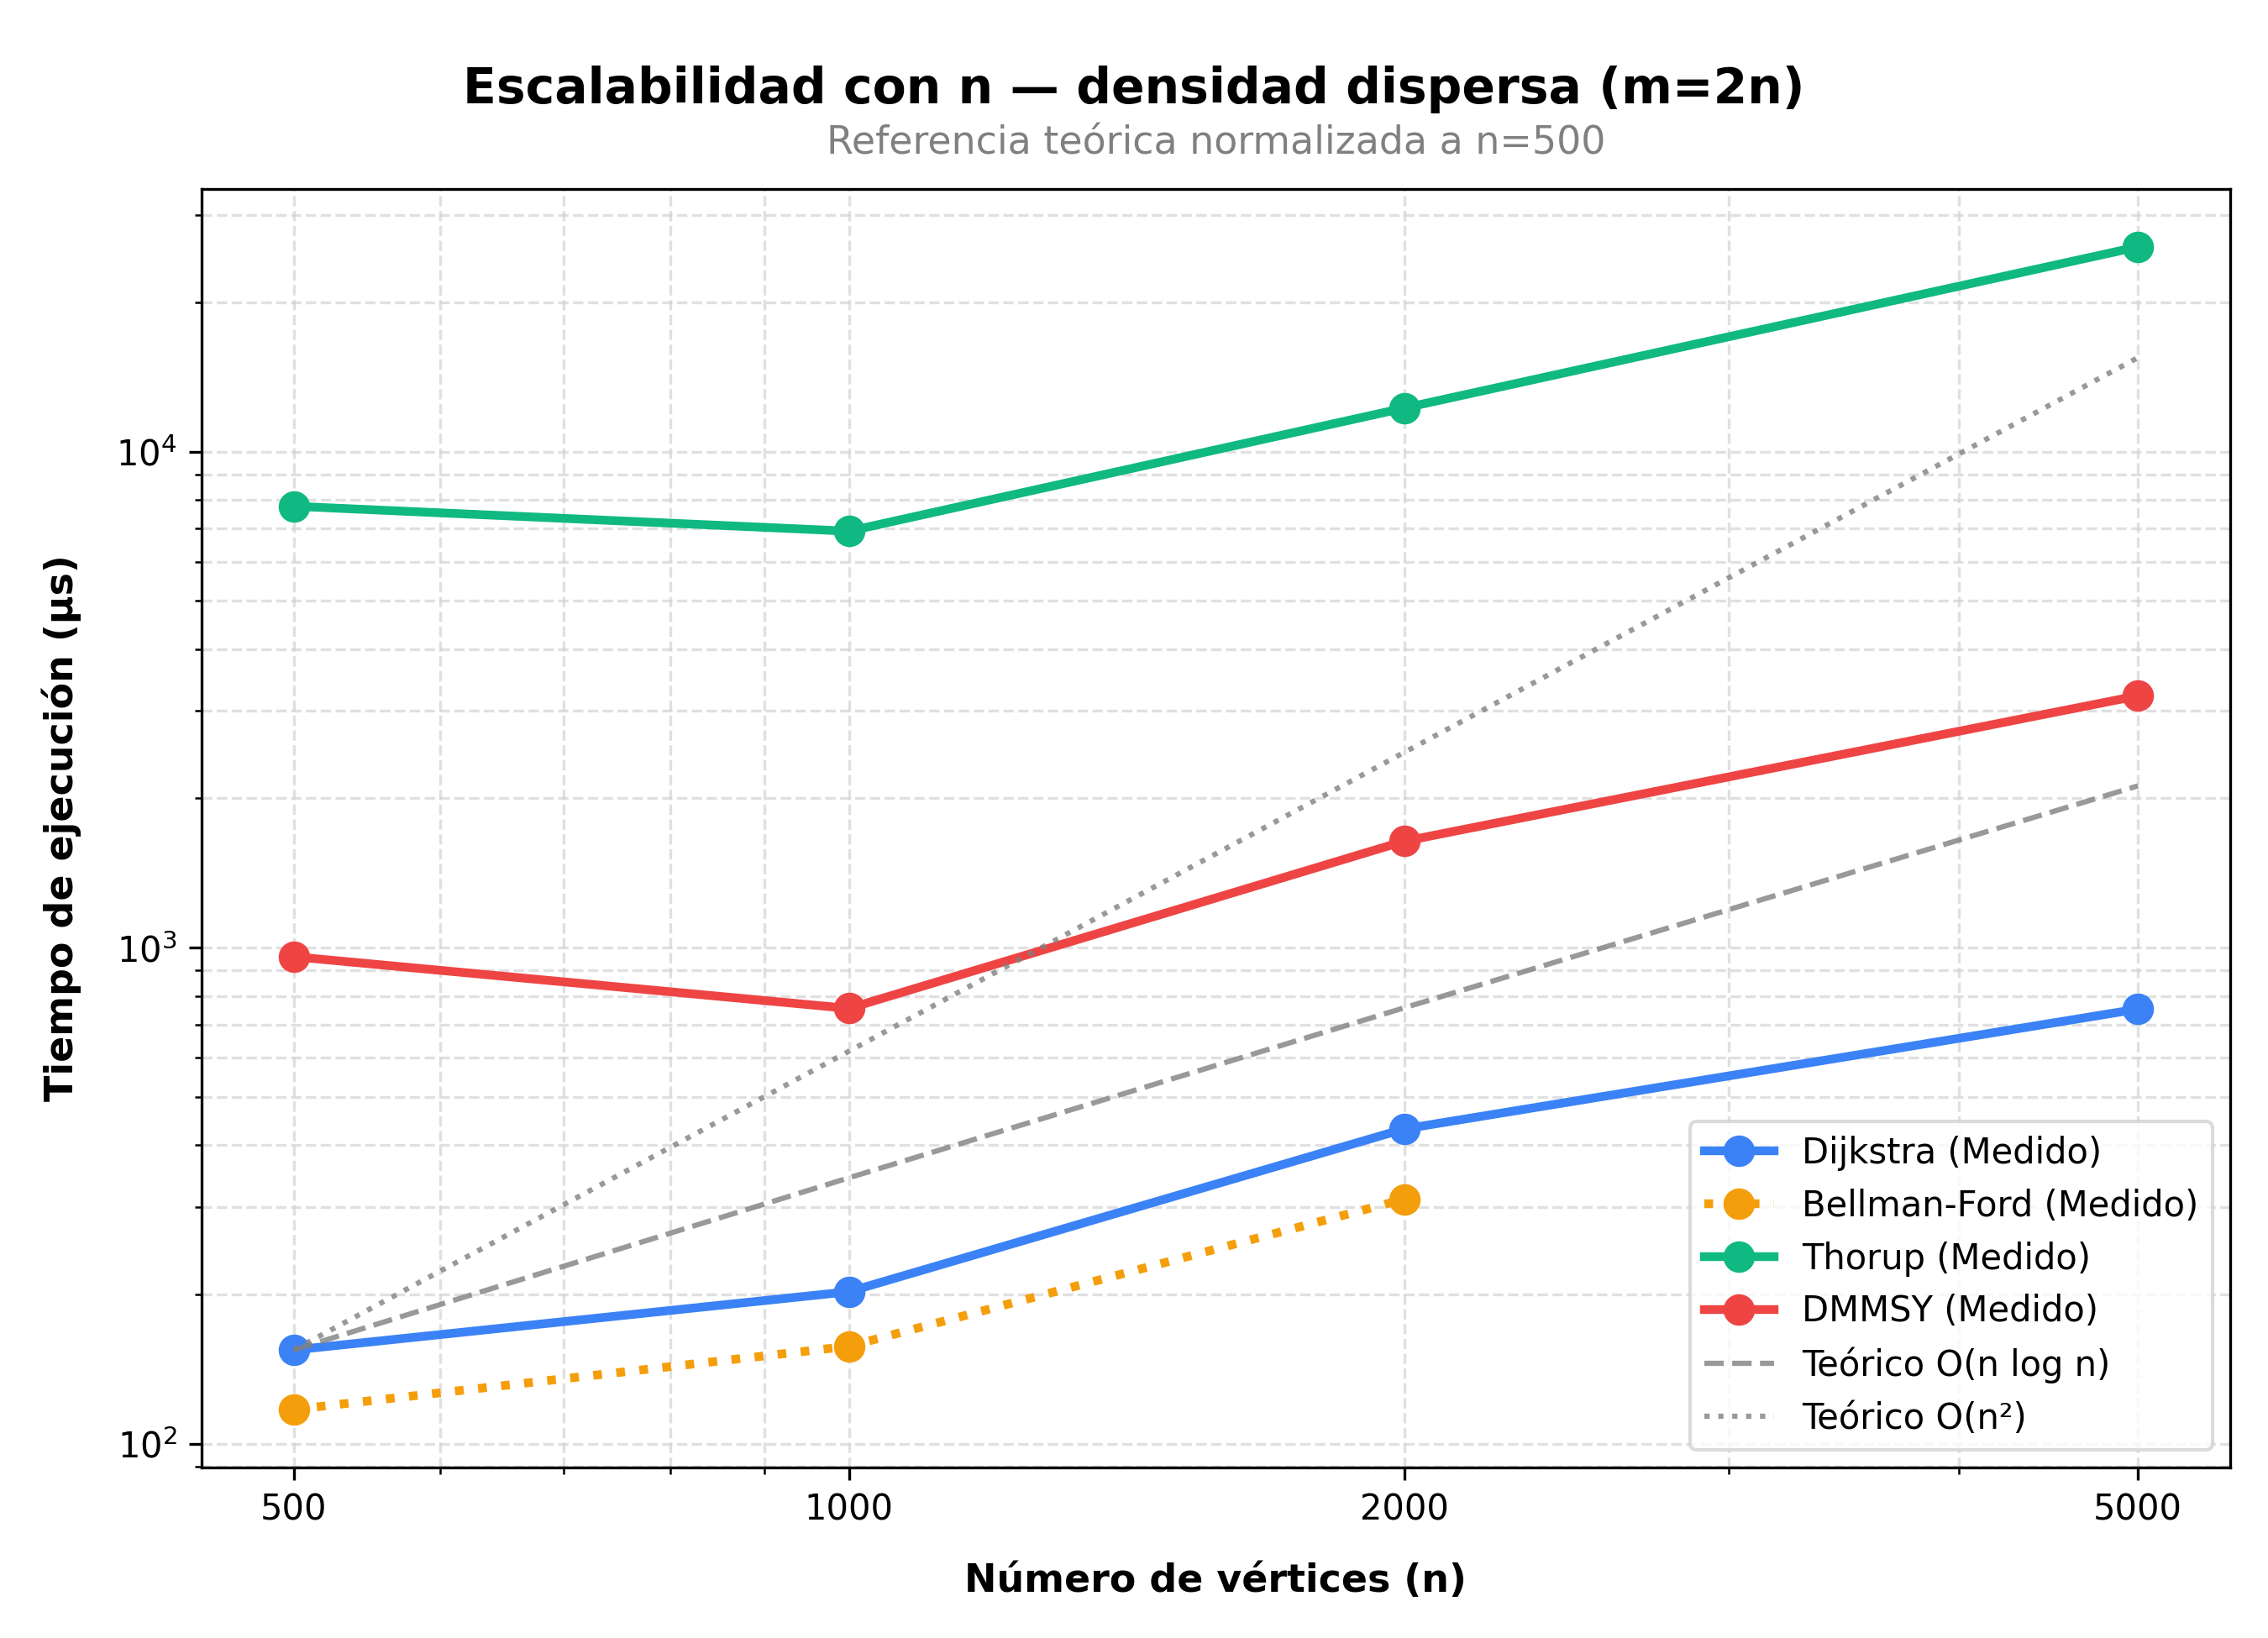
\includegraphics[width=7.5cm,height=5.8cm,keepaspectratio]{figuras/grafica4_scaling_n.png}
    \end{column}
  \end{columns}
\end{frame}

% ──────────────────────────────────────────────────────────────────────────────
\begin{frame}{Experimento 2 — Escalabilidad en $m$ ($n = 1{,}000$ fijo)}
  \begin{columns}[T]
    \begin{column}{0.52\textwidth}
      \small
      \textbf{Tabla de resultados:}
      \begin{center}
      \footnotesize
      \begin{tabular}{r r r r r}
        \toprule
        \rowcolor{azulUNSAAC!15}
        $m$ & Dijk. & BF & DMMSY & Thorup\\
        & ($\mu s$) & ($\mu s$) & ($\mu s$) & ($\mu s$)\\
        \midrule
        1\,000  & 53  & 1\,315 & 692 & 5\,334\\
        5\,000  & 301 & 200    & 740 & 7\,152\\
        10\,000 & 278 & 223    & 599 & 5\,208\\
        50\,000 & 631 & 559    & 658 & 4\,878\\
        100\,000& 619 & 857    & 793 & 5\,492\\
        200\,000& 838 & 1\,439 & 883 & 6\,245\\
        \bottomrule
      \end{tabular}
      \end{center}
      \vspace{0.2cm}
      \begin{itemize}\small
        \item \textbf{Cruce BF $\approx$ Dijkstra:} entre $m=5{,}000$ y $m=10{,}000$
        \item Thorup $\approx$ \textbf{constante} ($5{,}000$--$7{,}000\,\mu s$)
        \item DMMSY muestra convergencia suave con $m$
      \end{itemize}
    \end{column}
    \begin{column}{0.44\textwidth}
      \begin{tikzpicture}[scale=0.85]
        \begin{axis}[
          xlabel={$m$ (aristas)},
          ylabel={Tiempo ($\mu s$)},
          grid=major,
          legend style={font=\tiny,at={(0.02,0.98)},anchor=north west},
          xtick={1000,5000,10000,50000,100000,200000},
          xticklabels={1k,5k,10k,50k,100k,200k},
          x tick label style={font=\tiny,rotate=30},
          y tick label style={font=\tiny},
          width=6cm, height=5.5cm,
          ]
          \addplot[color=azulUNSAAC,mark=*,thick]
            coordinates{(1000,53)(5000,301)(10000,278)(50000,631)(100000,619)(200000,838)};
          \addlegendentry{Dijkstra}
          \addplot[color=orange!80!black,mark=square*,thick]
            coordinates{(1000,1315)(5000,200)(10000,223)(50000,559)(100000,857)(200000,1439)};
          \addlegendentry{Bellman-Ford}
          \addplot[color=verdeDark,mark=triangle*,thick]
            coordinates{(1000,692)(5000,740)(10000,599)(50000,658)(100000,793)(200000,883)};
          \addlegendentry{DMMSY}
          \addplot[color=rojoAlerta,mark=diamond*,thick]
            coordinates{(1000,5334)(5000,7152)(10000,5208)(50000,4878)(100000,5492)(200000,6245)};
          \addlegendentry{Thorup}
        \end{axis}
      \end{tikzpicture}
    \end{column}
  \end{columns}
\end{frame}

% ──────────────────────────────────────────────────────────────────────────────
\begin{frame}{Experimento 3 — Efecto de la Densidad ($n = 500$ fijo)}
  \begin{center}
  \small
  \begin{tabular}{l r r r r}
    \toprule
    \rowcolor{azulUNSAAC!20}
    \textbf{Etiqueta} & \textbf{Dijk.} & \textbf{BF} & \textbf{DMMSY} & \textbf{Thor.}\\
    & ($\mu s$) & ($\mu s$) & ($\mu s$) & ($\mu s$)\\
    \midrule
    muy disp. & \oktext{15}  & 366 & 1\,415 & 3\,218\\
    disperso  & 383 & \oktext{231} & 588 & 3\,367\\
    medio     & 348 & \oktext{157} & 470 & 2\,807\\
    \rowcolor{dorado!15}
    denso     & 683 & 570 & \highlight{533} & 2\,968\\
    \bottomrule
  \end{tabular}
  \end{center}
  \vspace{0.1cm}
  \begin{alertblock}{\small Hallazgo clave del Exp. 3}
    \small Para $m=50{,}000$ (densidad 20\%), DMMSY (\highlight{533~$\mu$s}) supera a
    Dijkstra (683~$\mu$s): \textbf{único escenario en Exps. 1--3} donde DMMSY gana.
  \end{alertblock}
\end{frame}

% ──────────────────────────────────────────────────────────────────────────────
\begin{frame}{Experimento 3 — Gráfico Tiempo vs. Densidad ($n = 500$)}
  \begin{center}
    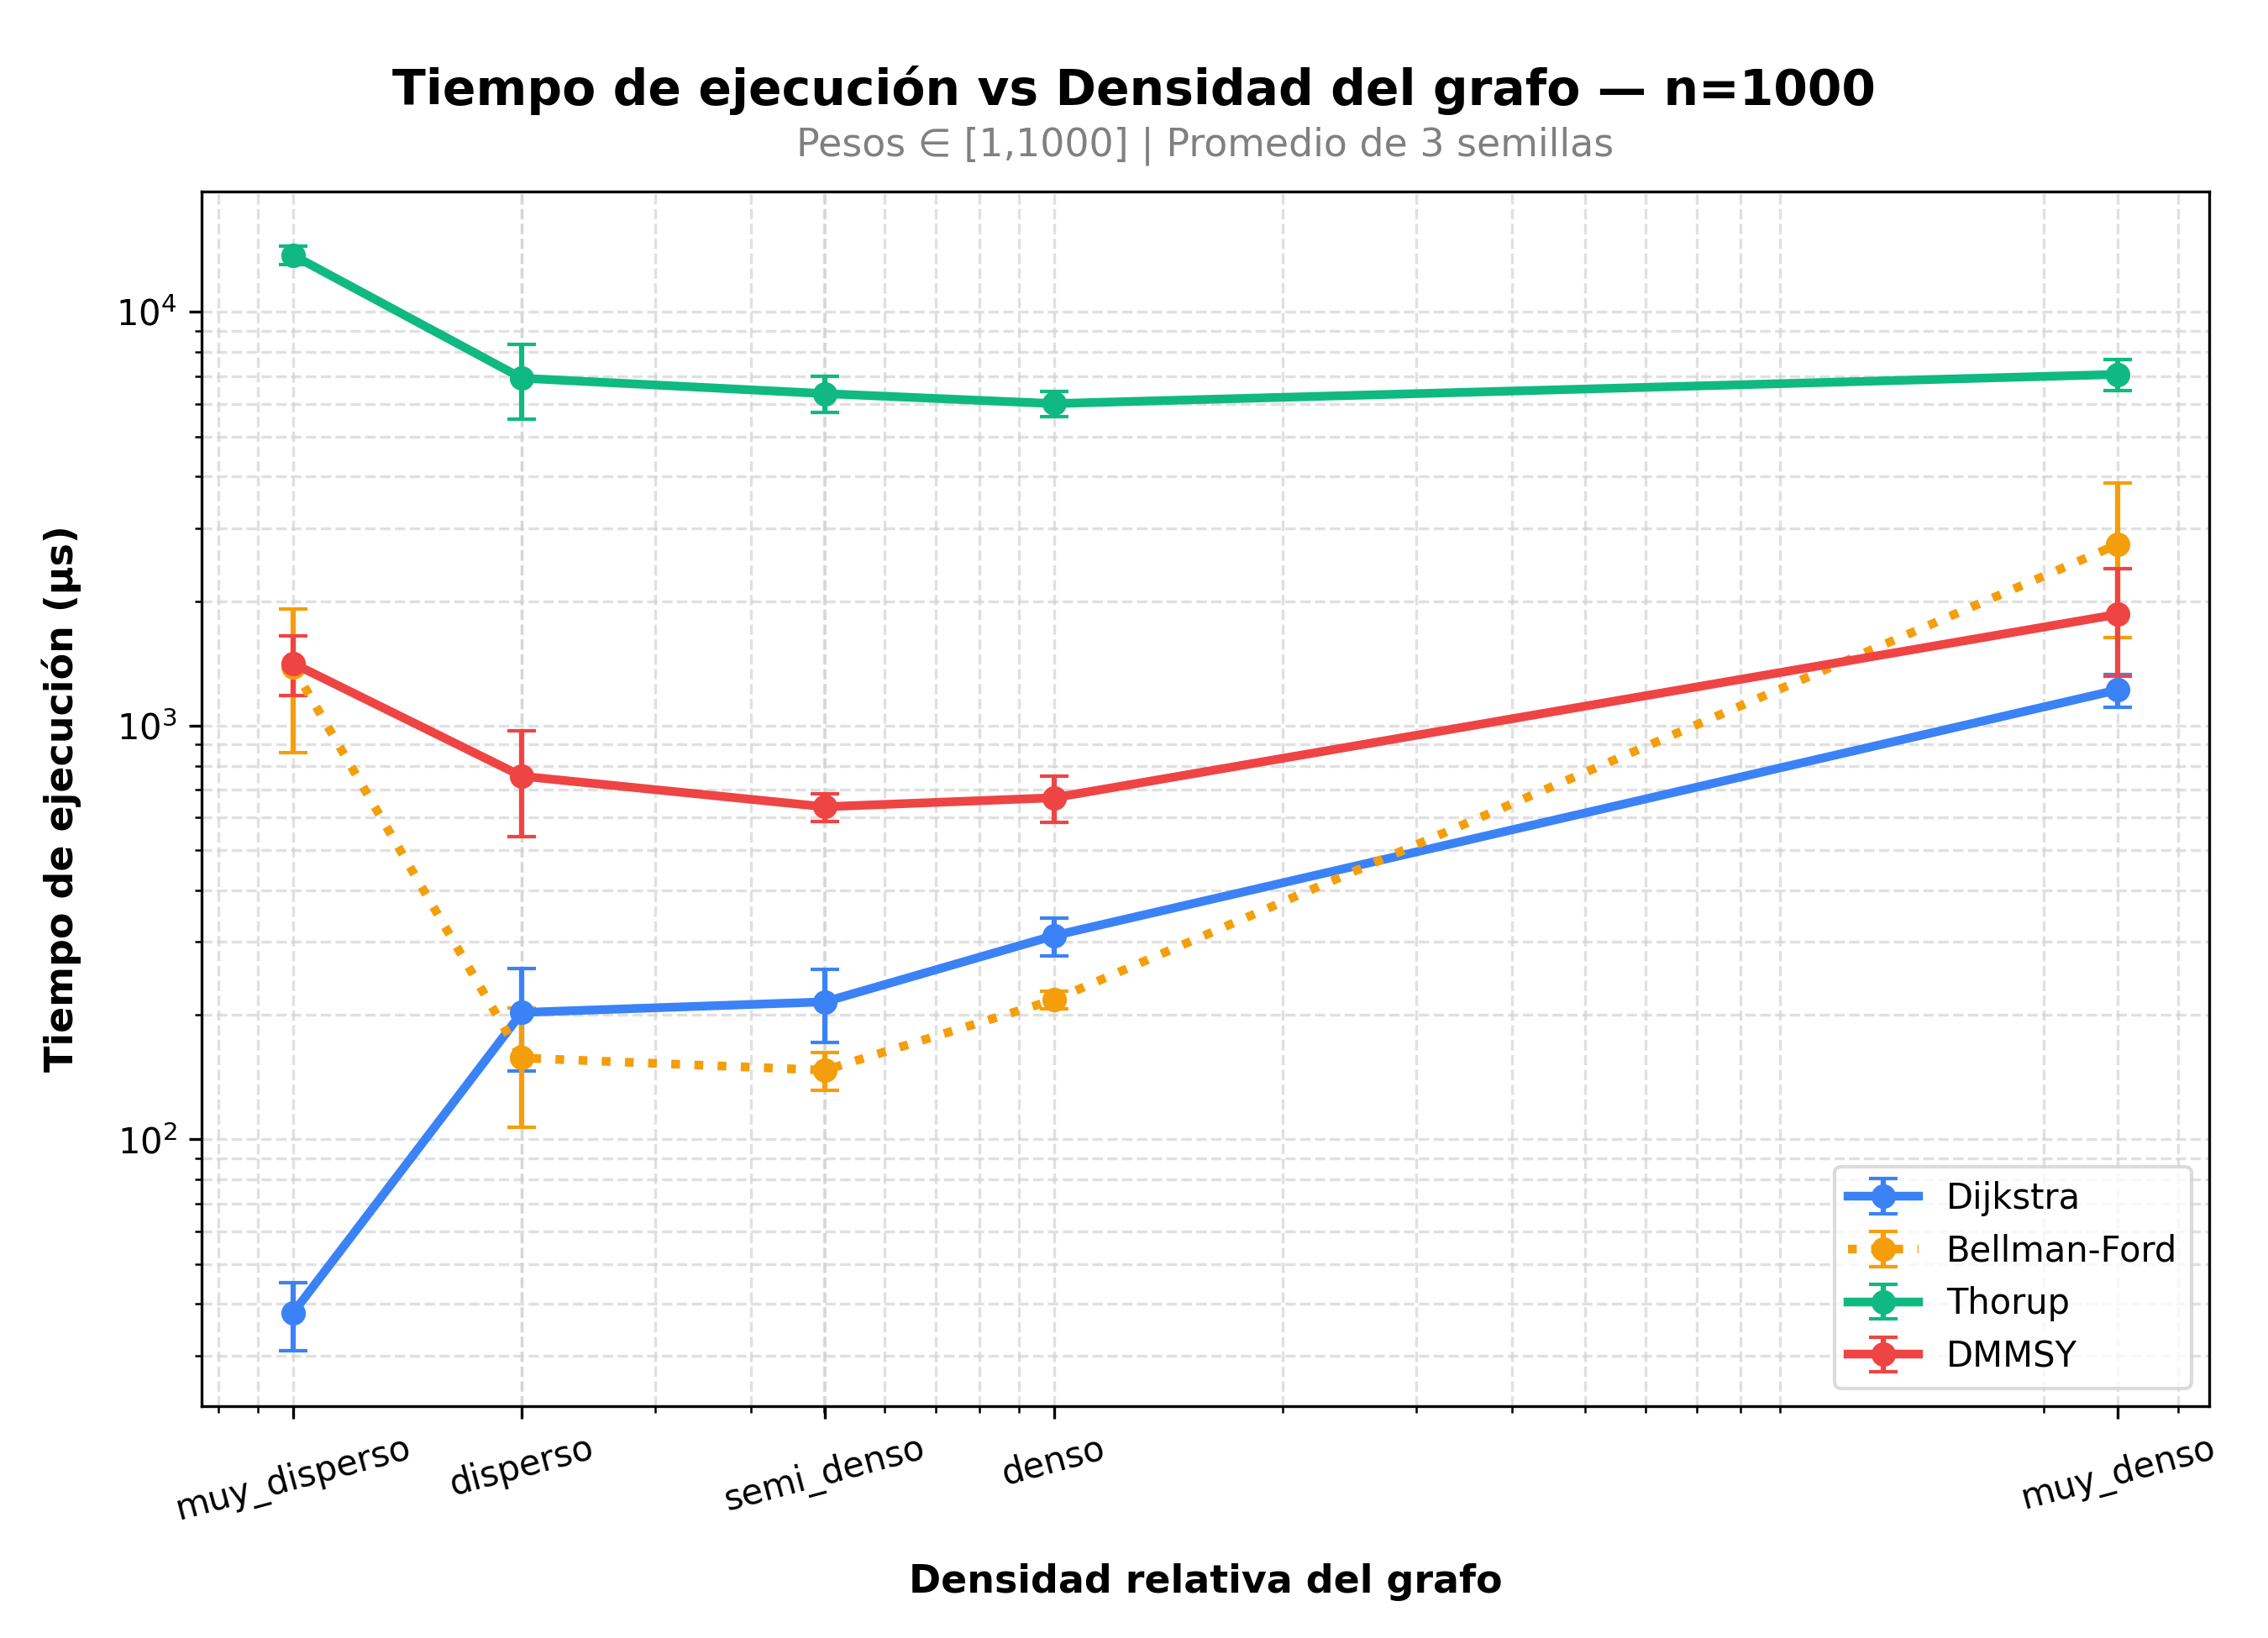
\includegraphics[width=11cm,height=7cm,keepaspectratio]{figuras/grafica1_tiempo_vs_densidad.png}
  \end{center}
\end{frame}

% ===============================================================================
\section{Resultados: Experimento 4 (Aporte Propio)}
% ===============================================================================

\begin{frame}{Experimento 4 — Diseño y Motivación}
  \begin{block}{Diseño factorial cruzado}
    $4\;\text{valores de }n \;\times\; 5\;\text{niveles de densidad}
    \;\times\; 3\;\text{semillas} = \mathbf{60}\;\text{mediciones}$
  \end{block}
  \vspace{0.2cm}
  \begin{columns}[T]
    \begin{column}{0.5\textwidth}
      \textbf{Parámetros:}
      \begin{itemize}\small
        \item $n \in \{500, 1{,}000, 2{,}000, 5{,}000\}$
        \item Densidades: muy\_disperso ($m\!=\!n$), disperso ($2n$),
          semi\_denso ($5n$), denso ($10n$), muy\_denso ($\lfloor n^2/4\rfloor$)
        \item Semillas: \{42, 123, 999\}
      \end{itemize}
    \end{column}
    \begin{column}{0.46\textwidth}
      \textbf{Objetivo:}
      \begin{itemize}\small
        \item Cuantificar el \textbf{impacto sistemático de la densidad}
        \item Identificar regiones del espacio $(n,\,m)$ donde cada algoritmo domina
        \item Verificar o refutar las cuatro hipótesis
        \item Proveer intervalos de confianza (media ± desv. est. sobre 3 semillas)
      \end{itemize}
    \end{column}
  \end{columns}
\end{frame}

% ──────────────────────────────────────────────────────────────────────────────
\begin{frame}{Exp. 4 — Tiempo vs. Densidad para $n = 1{,}000$}
  \begin{center}
    \small
    \begin{tabular}{l r r r r l}
      \toprule
      \rowcolor{azulUNSAAC!20}
      \textbf{Densidad} & \textbf{Dijkstra} & \textbf{BF} & \textbf{Thorup} & \textbf{DMMSY} & \textbf{Ganador}\\
      & ($\mu s\pm\sigma$) & ($\mu s\pm\sigma$) & ($\mu s\pm\sigma$) & ($\mu s\pm\sigma$) & \\
      \midrule
      muy\_disperso & $38.0\!\pm\!7.1$ & $1387.7\!\pm\!529$ & $13712\!\pm\!677$ & $1415\!\pm\!231$ & \oktext{Dijkstra}\\
      disperso      & $202.7\!\pm\!56$ & $157.3\!\pm\!50$   & $6912\!\pm\!1419$ & $754.7\!\pm\!216$ & \oktext{BF}\\
      semi\_denso   & $215.0\!\pm\!43$ & $147.0\!\pm\!16$   & $6344\!\pm\!632$  & $636.7\!\pm\!49$  & \oktext{BF}\\
      denso         & $310.7\!\pm\!33$ & $217.3\!\pm\!11$   & $6001\!\pm\!411$  & $669.3\!\pm\!85$  & \oktext{BF}\\
      muy\_denso    & $1220\!\pm\!111$ & $2742\!\pm\!1113$  & $7060\!\pm\!601$  & $1858\!\pm\!542$  & \oktext{Dijkstra}\\
      \bottomrule
    \end{tabular}
  \end{center}
  \vspace{0.2cm}
  \begin{columns}[c]
    \begin{column}{0.6\textwidth}
      \small
      \begin{itemize}
        \item \textbf{BF con terminación temprana} gana en densidades intermedias
          (hasta $\approx28\%$ más rápido que Dijkstra para semi\_denso)
        \item Thorup es \alerttext{consistentemente el más lento} (mín. $6{,}001\,\mu s$)
        \item En muy\_denso, BF vuelve a perder por el gran $m$
      \end{itemize}
    \end{column}
    \begin{column}{0.37\textwidth}
      \begin{tikzpicture}[scale=0.75]
        \begin{axis}[
          xlabel={Densidad},
          ylabel={Tiempo ($\mu s$)},
          xtick={1,2,3,4,5},
          xticklabels={M.D.,D.,S.D.,Den.,M.Den.},
          x tick label style={font=\tiny},
          y tick label style={font=\tiny},
          grid=major,
          legend style={font=\tiny,at={(0.98,0.98)},anchor=north east},
          width=5.5cm, height=4.5cm,
          ymode=log,
          ]
          \addplot[azulUNSAAC,mark=*,thick]
            coordinates{(1,38)(2,202.7)(3,215)(4,310.7)(5,1220)};
          \addlegendentry{Dijkstra}
          \addplot[orange!80!black,mark=square*,thick]
            coordinates{(1,1387.7)(2,157.3)(3,147)(4,217.3)(5,2742)};
          \addlegendentry{BF}
          \addplot[verdeDark,mark=triangle*,thick]
            coordinates{(1,1415)(2,754.7)(3,636.7)(4,669.3)(5,1858)};
          \addlegendentry{DMMSY}
        \end{axis}
      \end{tikzpicture}
    \end{column}
  \end{columns}
\end{frame}

% ──────────────────────────────────────────────────────────────────────────────
\begin{frame}{Exp. 4 — Mapa de Ganadores por $(n, \text{densidad})$}
  \begin{center}
  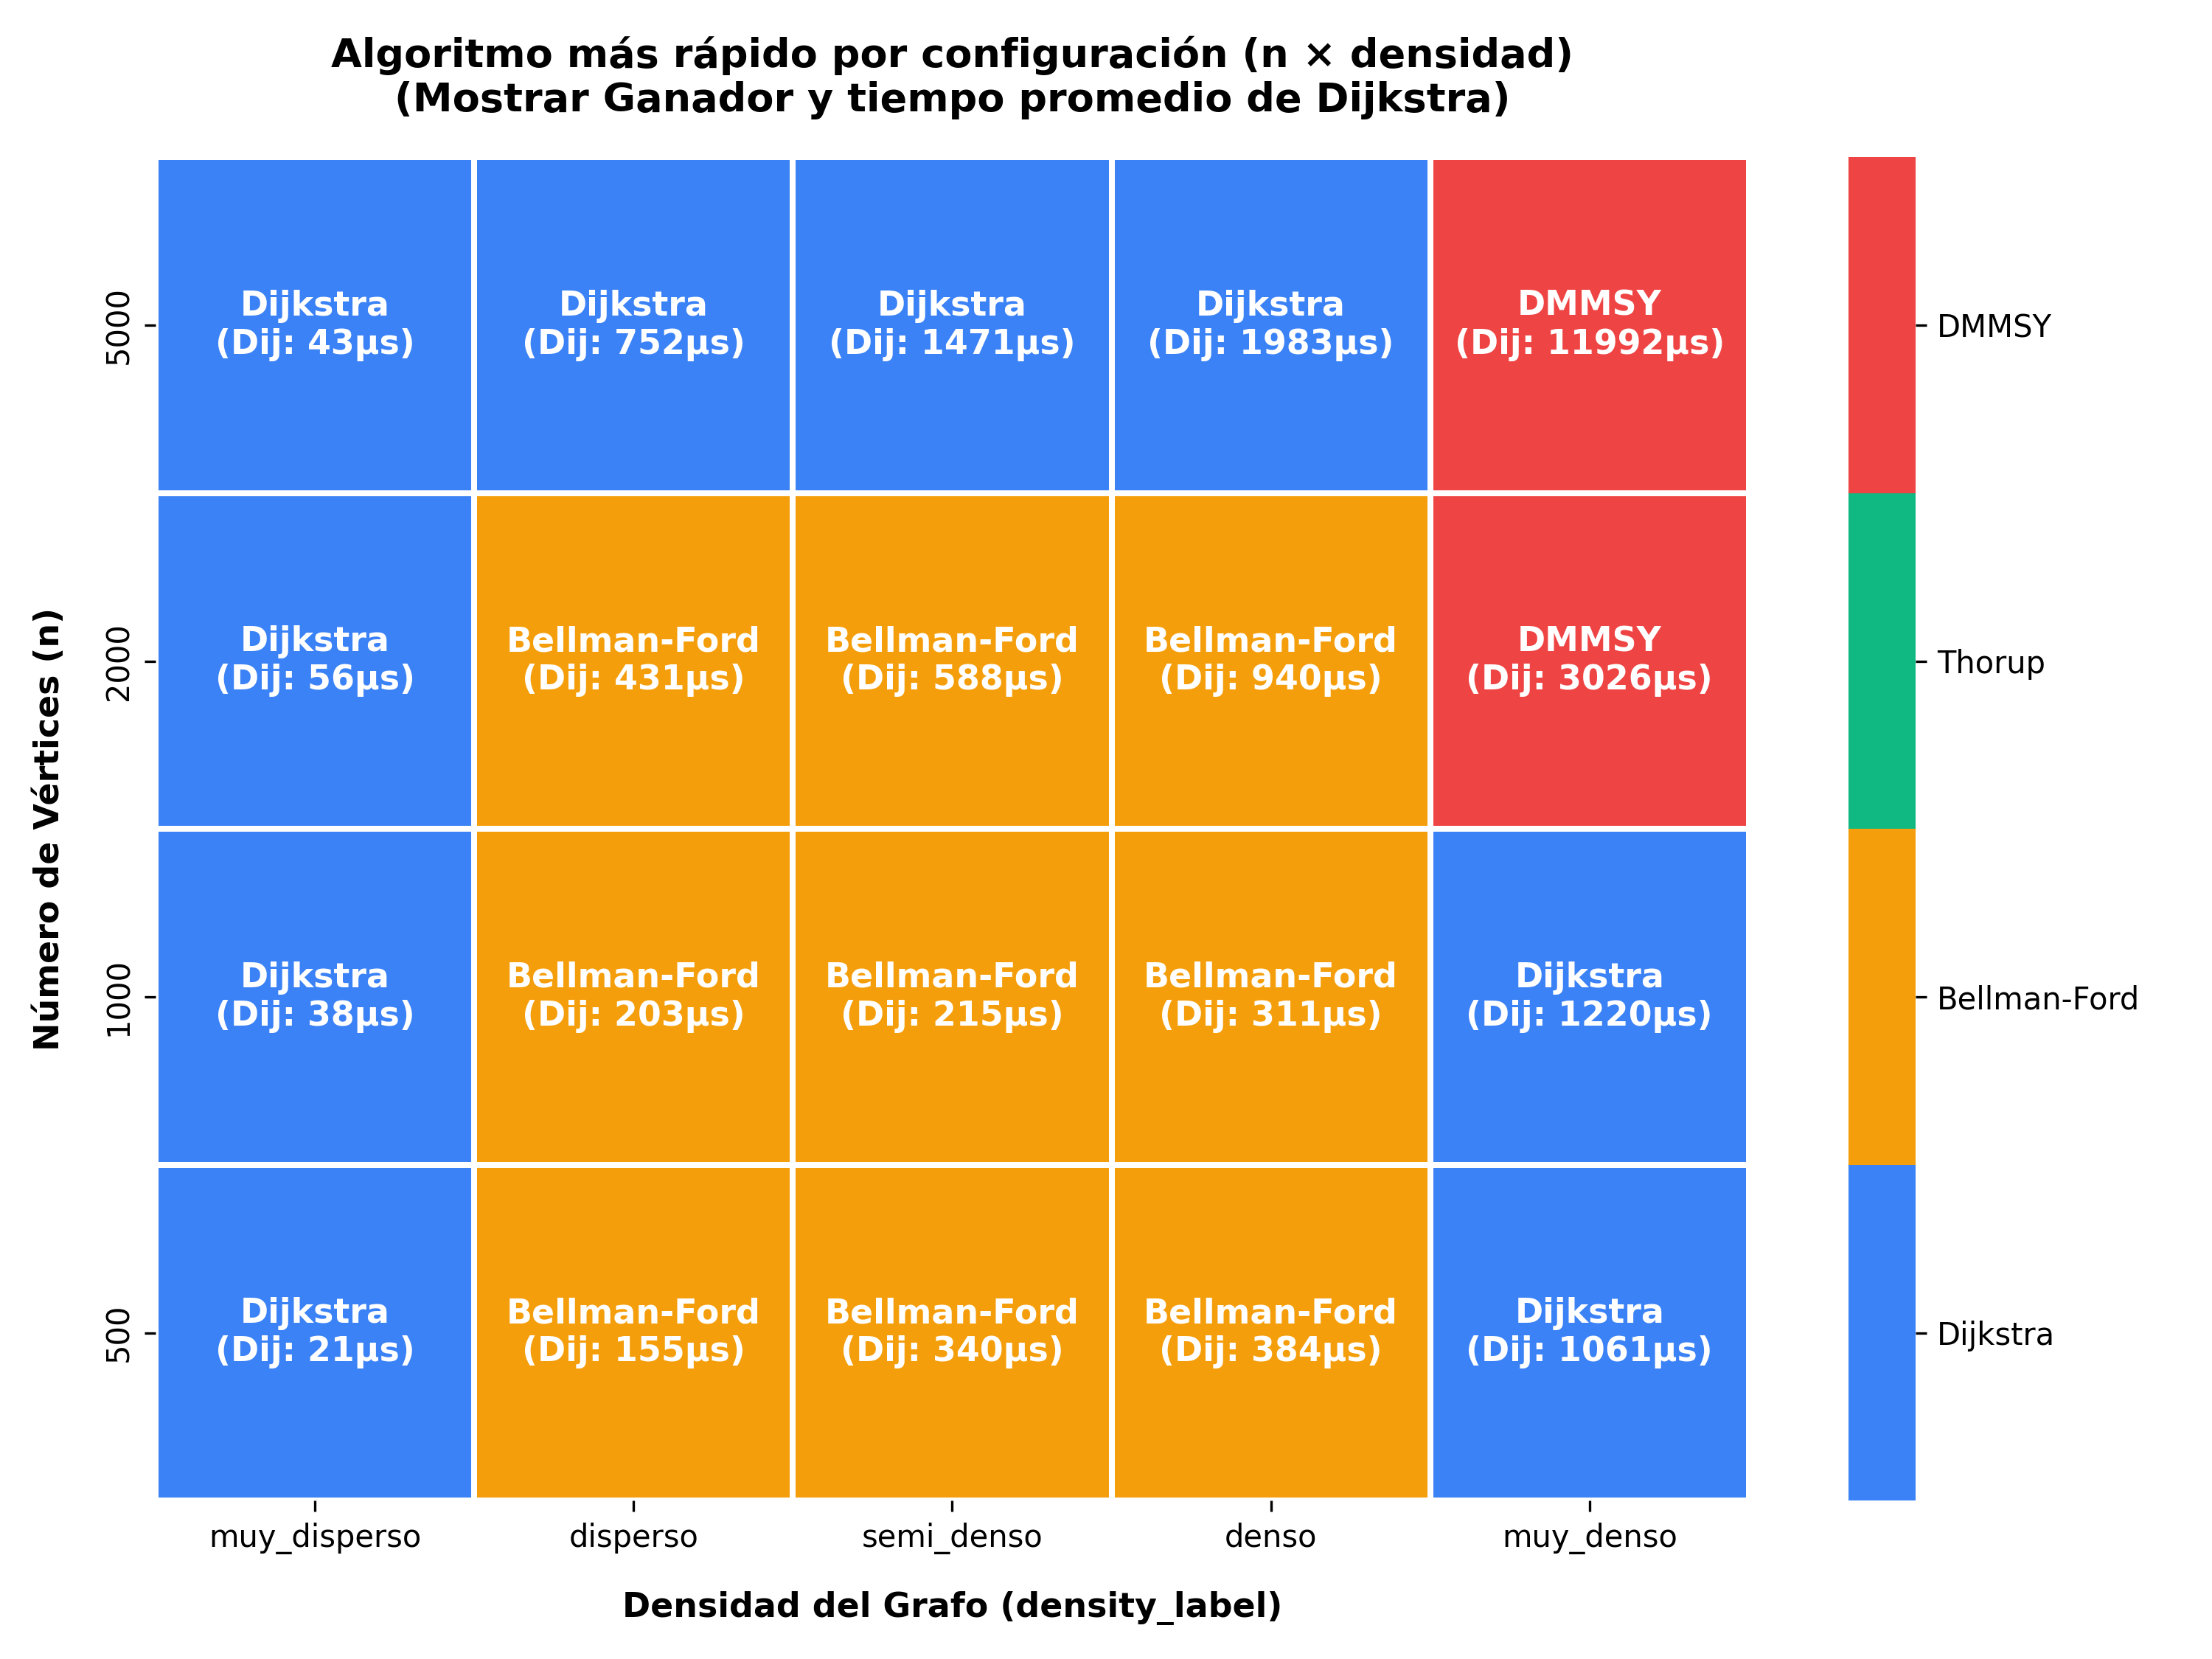
\includegraphics[width=11cm,height=7.5cm,keepaspectratio]{figuras/grafica3_heatmap_ganador.png}
  \end{center}
\end{frame}

% ──────────────────────────────────────────────────────────────────────────────
\begin{frame}{Exp. 4 — Interpretación del Mapa de Ganadores}
  \begin{columns}[c]
    \begin{column}{0.32\textwidth}
      \centering
      \colorbox{azulUNSAAC!25}{\strut\textbf{Dijkstra}}\\
      \vspace{0.3cm}
      \small muy\_disperso y muy\_denso ($n$ pequeño)
    \end{column}
    \begin{column}{0.32\textwidth}
      \centering
      \colorbox{orange!25}{\strut\textbf{Bellman-Ford}}\\
      \vspace{0.3cm}
      \small densidades intermedias, $n\leq2{,}000$
    \end{column}
    \begin{column}{0.32\textwidth}
      \centering
      \colorbox{verdeDark!25}{\strut\textbf{DMMSY}}\\
      \vspace{0.3cm}
      \small muy\_denso, $n\geq2{,}000$
    \end{column}
  \end{columns}
\end{frame}

% ──────────────────────────────────────────────────────────────────────────────
\begin{frame}{Exp. 4 — Operaciones de Relajación}
  \begin{block}{Observaciones clave}
    \begin{itemize}\small
      \item \textbf{Dijkstra, Thorup y DMMSY} realizan \emph{exactamente} el mismo
        número de relajaciones (curvas superpuestas)
      \item \textbf{Bellman-Ford} realiza entre \highlight{8× y 163×} más relajaciones
      \item La brecha se acentúa en grafos dispersos
      \item La ventaja de BF en tiempo viene de \textbf{operaciones más simples},
        no de menos relajaciones
    \end{itemize}
  \end{block}
  \vspace{0.15cm}
  \begin{alertblock}{\small Conclusión}
    \small El tiempo de BF en densidades intermedias se explica por la
    \textbf{terminación temprana}, no por un menor número de operaciones.
  \end{alertblock}
\end{frame}

% ──────────────────────────────────────────────────────────────────────────────
\begin{frame}{Exp. 4 — Gráfico de Operaciones de Relajación}
  \begin{center}
    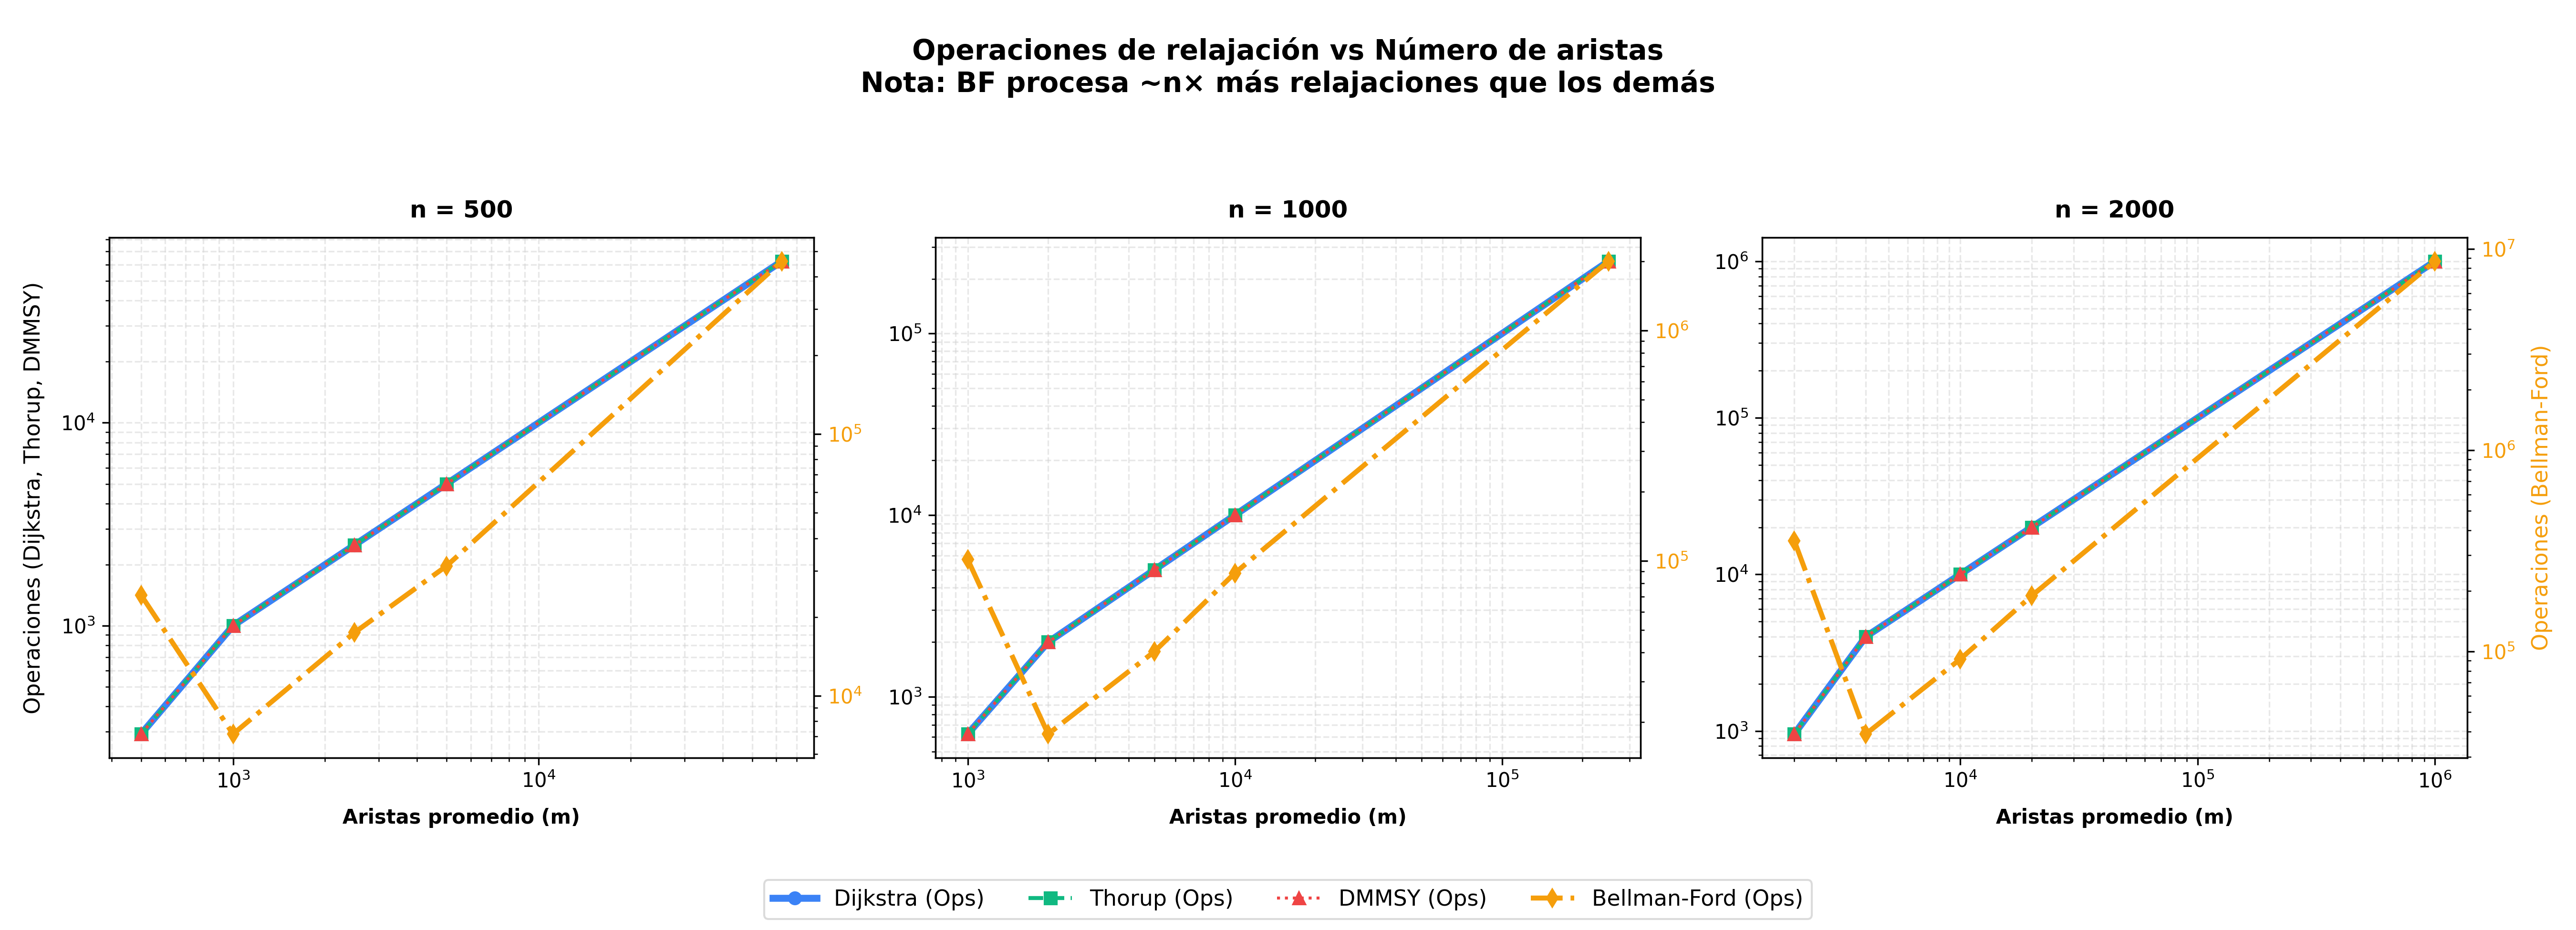
\includegraphics[width=15cm,height=10cm,keepaspectratio]{figuras/grafica2_ops_vs_m.png}
  \end{center}
\end{frame}

% ──────────────────────────────────────────────────────────────────────────────
\begin{frame}{Exp. 4 — Escalabilidad con $n$ (Densidad Dispersa, $m=2n$)}
  \begin{center}
  \small
  \begin{tabular}{r r r r r}
    \toprule
    \rowcolor{azulUNSAAC!15}
    $n$ & Dijk. ($\mu s$) & BF ($\mu s$) & DMMSY ($\mu s$) & Thor. ($\mu s$)\\
    \midrule
    500   & 154.7 & 117.3 & 959.3  & 7\,759\\
    1\,000 & 202.7 & 157.3 & 754.7  & 6\,912\\
    2\,000 & 431.3 & 311.3 & 1\,639 & 12\,236\\
    5\,000 & 752.3 & ---   & 3\,220 & 25\,858\\
    \bottomrule
  \end{tabular}
  \end{center}
  \vspace{0.2cm}
  \begin{itemize}\small
    \item Dijkstra crece $4.86\times$ de $n=500$ a $n=5{,}000$
      (factor teórico $\approx 13.7\times$): eficiencia de caché para $m$ pequeño
    \item DMMSY mejora de $n=500$ a $n=1{,}000$ por calibración de ancho $w_0$
    \item BF omitido para $n=5{,}000$ por coste cuadrático
  \end{itemize}
\end{frame}

% ──────────────────────────────────────────────────────────────────────────────
\begin{frame}{DMMSY en Alta Densidad: ¿Cuánto mejora a Dijkstra?}
  \begin{center}
  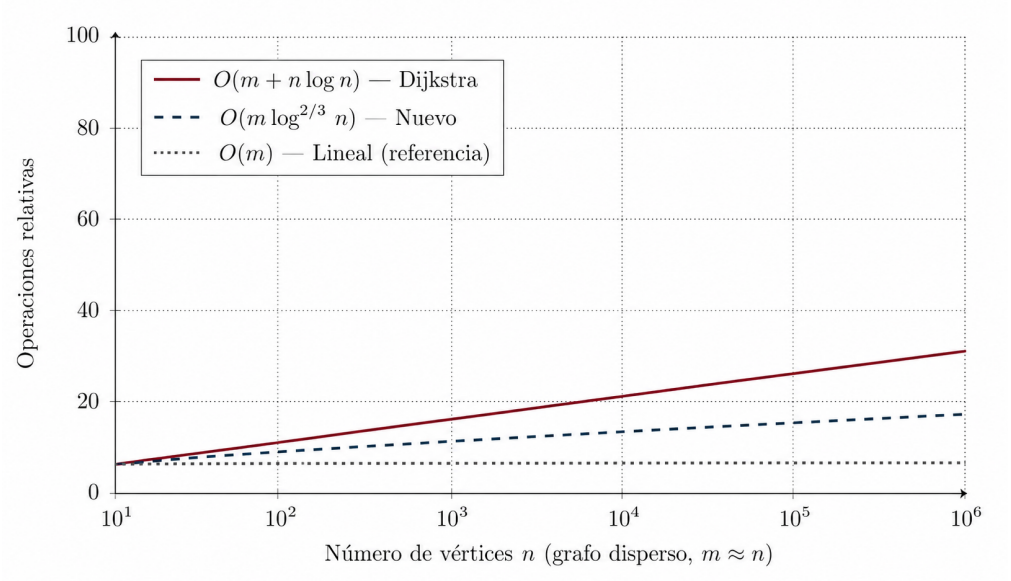
\includegraphics[width=10cm]{figuras/grafico_comparacion.png}
  \end{center}
  \begin{center}\small
    Para $n=2{,}000$: DMMSY tarda \highlight{2\,621~$\mu$s} vs Dijkstra \alerttext{3\,026~$\mu$s} \\
    Para $n=5{,}000$: DMMSY tarda \highlight{10\,171~$\mu$s} vs Dijkstra \alerttext{11\,992~$\mu$s} ($\approx15\%$ de mejora)
  \end{center}
\end{frame}

% ===============================================================================
\section{Verificación de Hipótesis}
% ===============================================================================

\begin{frame}{Verificación de las Cuatro Hipótesis}
  \begin{itemize}
    \setlength\itemsep{0.5em}

    \item[\oktext{$\checkmark$}]
    \textbf{H1 — CONFIRMADA.}
    Dijkstra es el ganador absoluto en grafos muy dispersos para todos los valores de $n$
    evaluados (38.0~$\mu$s para $n=1{,}000$, muy\_disperso).

    \item[\textcolor{orange!80!black}{!!}]
    \textbf{H2 — PARCIALMENTE CONFIRMADA.}
    BF es inviable para $n>2{,}000$, pero para $n\leq2{,}000$ y densidades intermedias
    \textbf{supera a Dijkstra} (157.3~$\mu$s vs 215.0~$\mu$s para semi\_denso).
    La hipótesis subestimó la eficiencia de la terminación temprana.

    \item[\oktext{$\checkmark$}]
    \textbf{H3 — CONFIRMADA.}
    Thorup es el más lento en todos los escenarios (mínimo 6\,001~$\mu$s para $n=1{,}000$, denso).

    \item[\oktext{$\checkmark$}]
    \textbf{H4 — CONFIRMADA.}
    DMMSY supera a Dijkstra en grafos de muy alta densidad y $n\geq2{,}000$
    (2\,621~$\mu$s vs 3\,026~$\mu$s para $n=2{,}000$, muy\_denso).
  \end{itemize}
\end{frame}

% ===============================================================================
\section{Fundamentos Teóricos: El Algoritmo DMMSY}
% ===============================================================================

\begin{frame}{¿Por qué \complejidad{m\log^{2/3}n} es un avance?}
  \begin{columns}[T]
    \begin{column}{0.48\textwidth}
      \begin{block}{Dijkstra (estándar)}
        \begin{equation*}
          T_{\text{Dijkstra}} = \mathcal{O}(m + n\log n)
        \end{equation*}
        Cuello de botella: la cola de prioridad global obliga a \textbf{ordenar todos los vértices}.
      \end{block}
      \vspace{0.2cm}
      \begin{alertblock}{Nuevo: DMMSY 2025}
        \begin{equation*}
          T_{\text{DMMSY}} = \mathcal{O}(m\log^{2/3}n)
        \end{equation*}
        Primer avance \textbf{determinista} significativo en $>20$ años.
      \end{alertblock}
    \end{column}
    \begin{column}{0.48\textwidth}
      \textbf{Ideas clave del paper:}
      \begin{enumerate}\small
        \item \textbf{Descomposición jerárquica:} $K=\lceil\log^{2/3}n\rceil$ niveles
        \item \textbf{Evitar ordenamiento global:} actualizaciones locales por región
        \item \textbf{Jerarquía de cubetas:} acceso $\mathcal{O}(1)$ al mínimo local
        \item \textbf{Aproximaciones multi-escala:} combina soluciones de distintos niveles
      \end{enumerate}
      \vspace{0.2cm}
      \begin{exampleblock}{\small Comparación teórica}
        \scriptsize
        Para $n=10^6$: $\log n\approx20$, $\log^{2/3}n\approx7.4$.\\
        En grafos dispersos ($m=\mathcal{O}(n)$): DMMSY ahorra $\approx 63\%$ en factor log.
      \end{exampleblock}
    \end{column}
  \end{columns}
\end{frame}

% ──────────────────────────────────────────────────────────────────────────────
\begin{frame}{Comparación Conceptual: Dijkstra vs. DMMSY}
  \begin{center}
  \scriptsize
  \begin{tabular}{l C{3.0cm} C{3.0cm}}
    \toprule
    \rowcolor{azulUNSAAC!20}
    \textbf{Aspecto} & \textbf{Dijkstra} & \textbf{DMMSY}\\
    \midrule
    Enfoque            & Secuencial voraz     & Basado en jerarquía\\
    Selección vértice  & Mínimo global (heap) & Mínimo local por nivel\\
    Ordenamiento       & Global de $V$        & Evita ordenamiento completo\\
    Modelo             & Comparación y suma   & Comparación y suma\\
    Pesos negativos    & No                   & No\\
    Complejidad        & $\mathcal{O}(m+n\log n)$ & $\mathcal{O}(m\log^{2/3}n)$\\
    Ventaja            & Simplicidad, constantes bajas & Mejor asintótica\\
    Desventaja         & Factor $\log$ inevitable & Alta complejidad de impl.\\
    \bottomrule
  \end{tabular}
  \end{center}
  \vspace{0.15cm}
  \begin{center}
    \footnotesize\textit{Nota:} la implementación educativa de DMMSY degenera en el Algoritmo de Dial
    de un nivel ($w_0=1$); no implementa la jerarquía completa ni las herramientas algebraicas del paper.
  \end{center}
\end{frame}

% ===============================================================================
\section{Conclusiones y Trabajo Futuro}
% ===============================================================================

\begin{frame}{Conclusiones Principales}
  \begin{enumerate}
    \setlength\itemsep{0.45em}
    \item \textbf{Dijkstra lidera en grafos dispersos} (\complejidad{m+n\log n} con constantes bajas):
      imbatible para $m=\mathcal{O}(n)$.

    \item \textbf{Bellman-Ford es competitivo en densidades intermedias} gracias a
      terminación temprana: supera a Dijkstra para $m\in[2n,\,10n]$ con $n\leq2{,}000$.

    \item \textbf{Thorup tiene alto overhead constante} ($>6{,}000\,\mu$s en todos los
      escenarios): impracticable en la implementación educativa.

    \item \textbf{DMMSY muestra promesa en grafos muy densos:} mejora $\approx15\%$
      sobre Dijkstra para $n\geq2{,}000$ y muy\_denso.

    \item \textbf{La densidad es el factor crítico:} el espacio $(n,\,m)$ tiene regiones de dominio
      bien diferenciadas para cada algoritmo.
  \end{enumerate}
\end{frame}

% ──────────────────────────────────────────────────────────────────────────────
\begin{frame}{Recomendaciones de Uso y Trabajo Futuro}
  {\small
  \begin{columns}[T]
    \begin{column}{0.48\textwidth}
      \begin{block}{$\mapsto$~Guía de selección}
        \begin{tabular}{@{}ll@{}}
          $m \leq 2n$ & $\Rightarrow$ \textbf{Dijkstra}\\[2pt]
          $m \in [2n,10n], n\!\leq\!2k$ & $\Rightarrow$ \textbf{BF}\\[2pt]
          $m > 10n, n\!\geq\!2k$ & $\Rightarrow$ \textbf{DMMSY}\\[2pt]
          Prod. simple & $\Rightarrow$ \textbf{Dijkstra}\\
        \end{tabular}
      \end{block}
    \end{column}
    \begin{column}{0.48\textwidth}
      \begin{exampleblock}{$\rightarrow$~Trabajo futuro}
        \begin{enumerate}\tiny
          \item Implementar DMMSY completo (jerarquía $K$ niveles)
          \item Algoritmos híbridos (Dijkstra + DMMSY adaptativos)
          \item Evaluación en grafos reales (OSM, SNAP)
          \item Versiones paralelas / GPU
          \item Análisis de impacto de caché y SIMD
        \end{enumerate}
      \end{exampleblock}
    \end{column}
  \end{columns}
  \vspace{0.25cm}
  \begin{alertblock}{\tiny Limitaciones conocidas}
    Implementaciones de Thorup y DMMSY son educativas (versiones simplificadas).
    Experimentos monohilo en hardware de escritorio; sin validación en grafos reales.
  \end{alertblock}
  }
\end{frame}

% ── Diapositiva final ─────────────────────────────────────────────────────────
{
\setbeamertemplate{headline}{}
\begin{frame}[plain]
  \begin{tikzpicture}[remember picture,overlay]
    \fill[azulUNSAAC] (current page.south west) rectangle (current page.north east);
    \fill[dorado] ([yshift=-0.5cm]current page.north west) rectangle
      ([yshift=-0.9cm]current page.north east);
  \end{tikzpicture}
  \begin{center}
    \vspace{1.8cm}
    {\color{white}\LARGE\bfseries¡Gracias!}\\[0.5cm]
    {\color{dorado}\large Caminos Más Cortos con Fuente Única}\\[0.3cm]
    {\color{white!80}\small Bustinza · Mayhuire · Estacio · Salcedo}\\[0.2cm]
    {\color{white!70}\small UNSAAC --- Algoritmos Avanzados --- Junio 2026}\\[0.6cm]
    {\color{white!60}\small$\triangleright$~224867@unsaac.edu.pe \quad 231445@unsaac.edu.pe}\\
    {\color{white!60}\small\phantom{$\triangleright$}~200822@unsaac.edu.pe \quad 200886@unsaac.edu.pe}
  \end{center}
\end{frame}
}

\end{document}
